\documentclass[12pt, a4paper, oneside]{ctexart}
\usepackage{graphicx}

\title{Uniswap简明导论}
\author{Splendor White}
\date{\today}

\begin{document}

\maketitle

\section{简介}

Uniswap 是以太坊区块链上的一个去中心化交易所。它既表现出与传统中心化交易所不同的特性,又是去中心化交易所的典型代表。了解其基本运行机制,是认识去中心化金融的基础。

与传统的中心化交易所不同,Uniswap 的交易不需要订单簿,而是由自动做市商根据恒定乘积公式对流动性池进行动态调整,满足交易者的交易需求。流动性提供者可以向流动性池中添加流动性,降低交易者的滑点,并按照份额赚取流动性费用。

Uniswap 是一个不断发展的交易协议。在 Uniswap V2 中,任意交易对、安全的价格预言机、闪电兑等功能得以实现。在 Uniswap V3 中,集中流动性的引入大大提高了资金利用率。在即将上线的 Uniswap V4 中,挂钩、单例、闪电记账等新元素使得合约可以更加灵活地定制化。

\section{订单簿与自动做市商}

在传统的金融交易过程中,一部分买者和卖者需要在一个公共订单簿(Order Book)上给出自己的买进报价(Bid)或卖出报价(Ask),这类交易者被称为挂单者(Maker)。其他的买者和卖者可以在订单簿中找到自己心仪的报价,并付给相应的商品或货币,从而完成交易,这类交易者被称为吃单者(Taker)。

\begin{figure}[htbp]
    \centering
    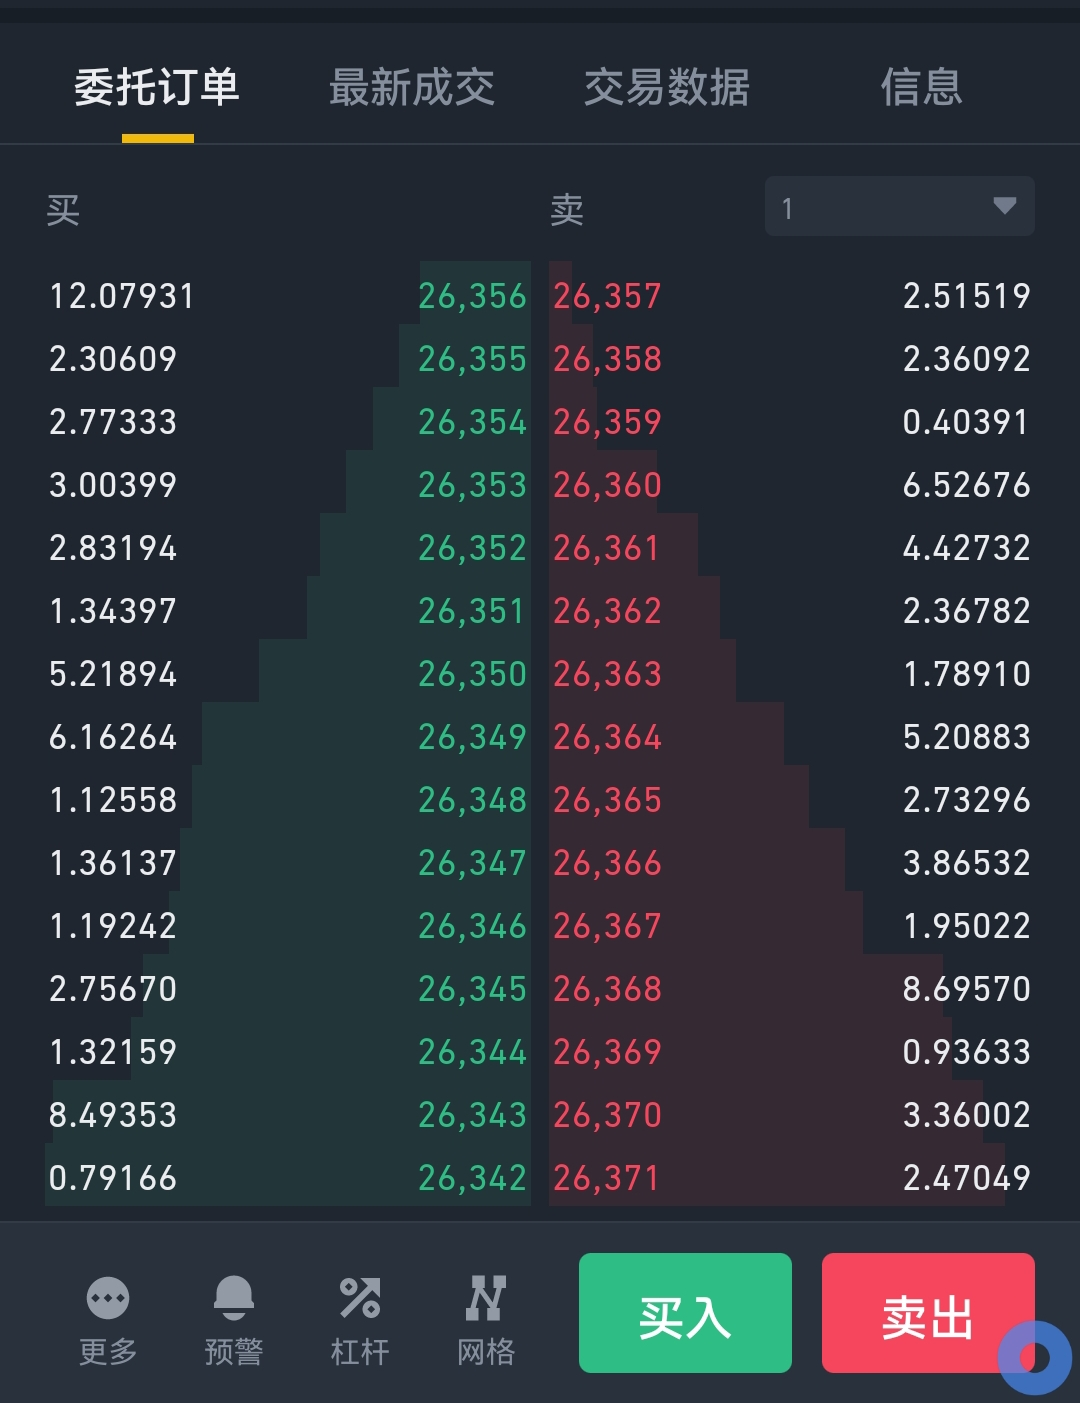
\includegraphics[width=8cm]{订单簿示意图.jpg}
    \caption{订单簿示意图}
\end{figure}

这种交易方式能够确定每一笔订单的成交价格和成交数量,并使得市场深度一目了然。

\end{document}

